\documentclass[
	%a4paper, % Use A4 paper size
	letterpaper, % Use US letter paper size
]{jdf}

\usepackage{multicol}

\addbibresource{references.bib}

\author{Steven Billington}
\email{sbillington3@gatech.edu}
\title{Homework \#2}

\begin{document}
%\lsstyle

\maketitle

%\begin{abstract}
%	Welcome to Joyner Document Format (JDF) v2.2! JDF is primarily intended to standardize page lengths while ensuring readability. Note that you are required to use JDF for all written assignments, but we will not perform explicit formatting checks. So, while improper formatting may be subject to penalties, you should not worry too much about whether your submission conforms to every minute detail; the most important elements are margins, font, font sizes, and line spacing. Just make a copy of one of the provided templates and replace its contents with your own, using the built-in paragraph styles.\footnote{Here are instructions for \href{https://support.office.com/en-us/article/Video-Using-Styles-in-Word-9db4c0f4-2754-4294-9758-c14a0abd8cfa}{Microsoft Word}, \href{https://support.apple.com/guide/pages/intro-to-paragraph-styles-tanaa39b0aa3/mac}{Apple Pages}, and \href{https://www.bazroberts.com/2016/04/19/google-docs-paragraph-styles-headings/}{Google Docs}.} If you do so, you do not need to verify that the style was followed.
%\end{abstract}

\section{Question \#1 - What is a Sandwich?}
\subsection{Billington Based Classification}
What is a sandwich? Is a hotdog a sandwich? I have been given a list of dishes and need to decide whether or not they are sandwiches. This will assist in helping me classify whether a hotdog is a sandwich.
\begin{multicols}{2}
\small
\begin{itemize}
    \item BLT on white bread. Sandwich.
    \item Hamburger. Sandwich
    \item Turkey and Swiss on a Potato roll. Sandwich.
    \item Meatball sub. Sandwich.
    \item Tuna Salad on brioche. Sandwich.
    \item Chicken Wrap. Not a Sandwich.
    \item Chip Butty. Sandwich.
    \item Burrito. Not a Sandwich.
    \item Ice Cream Sandwich. Not a Sandwich
    \item Grilled Cheese. Not a Sandwich.
    \item Turkey Hero. Sandwich.
    \item Ice Cream Taco. Not a Sandwich.
    \item Vada Pav. Not a Sandwich.
    \item Toast. Not a Sandwich.
    \item Cheese Quesadilla. Not a Sandwich.
    \item Toaster Strudel. Not a Sandwich.
    \item Veggie Burger. Sandwich.
    \item Klondike Bar. Not a Sandwich.
    \item Egg \& Cheese Biscuit. Not a Sandwich.
    \item Buttered Biscuit. Not a Sandwich.
    \item Gyro. Not a Sandwich.
    \item Sushi rolls. Not a Sandwich.
    \item Patty Melt. Sandwich.
    \item Calzone. Not a Sandwich.
    \item Sloppy Joe. Sandwich.
\end{itemize}
\end{multicols}
%Prior to beginning this question, consider one of the great internet debates of our time: what is a sandwich? First, take the following list of dishes and decide whether each one is a sandwich. In your assignment, start with a list of which of these you consider sandwiches, and which you do not. If you are unfamiliar with any of these types of sandwich, you should be able to Google them and find out what they are.
%BLT on white bread; hamburger; turkey and swiss on potato roll; meatball sub; tuna salad on brioche; chicken wrap; chip butty; burrito; ice cream sandwich; grilled cheese; turkey hero; ice cream taco; vada pav; toast; cheese quesadilla; toaster strudel; veggie burger; Klondike bar; egg \& cheese biscuit; buttered biscuit; gyro; sushi rolls; patty melt; calzone; sloppy joe.
\subsection{Incremental Concept Learning}
The potential series of sandwiches that I will use to demonstrate Incremental Concept Learning are "BLT on White Bread", "Patty Melt", "Ice Cream Sandwich", and "Chicken Wrap". Starting with the initial sandwich on that list of four, I created the following rudimentary diagram (Figure 1) describing a rudimentary concept of a sandwich. It is a bread object supporting a filling or middle layer of vegetables and meats which then supports another bread object. From there, we move to Patty Melt. A Patty Melt includes the middle layer of meat, but may not require vegetables. Also a Patty Melt typically includes cheese of some sort as a part of the middle layer. We will generalize from the initial diagram in Figure 1 to a more inclusive definition seen in Figure 2 where the middle layer becomes "Not Bread" (Close-interval heuristic to include everything but bread). But what about Ice Cream Sandwiches? I did not consider them sandwiches so some additional logic is missing here. 

\begin{figure}[h]
	\centering
	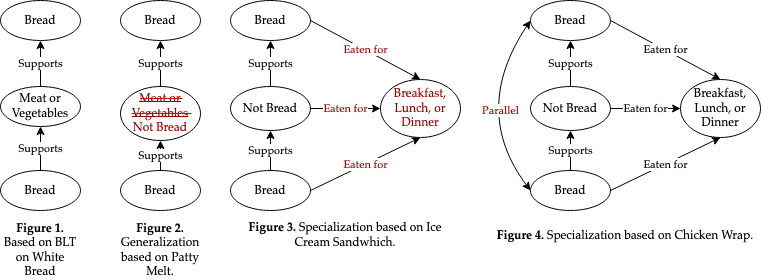
\includegraphics{SandwichFiguresCorrection.jpg}
	\label{fig:flowchart}
\end{figure}

From Figure 2 to Figure 3 I add a different node, a "meal" node is included where the meal is breakfast, lunch, or dinner. This specialization will exclude ice cream sandwiches since an ice cream sandwich is not a meal for breakfast, lunch or dinner. Finally we move to the Chicken Wrap, which is not a Sandwich. From here we will include a new relationship (Figure 4) between the two nodes of Bread that state that the flat portions of the bread to be parallel from one another. This specialization, a require link heuristic, would eliminate any configurations of wraps where a wrap is definitely not parallel from itself or any other wrap around it since it they touch.

Is there any sandwich type that will break the mold from the long list above? A Grilled Cheese would violate the current model since it meets all standards described but is not a sandwich and require additional specialization in order to eliminate as an option.
%Once you’ve labeled each of those, illustrate the process of incremental concept learning using a series of potential sandwiches. Construct a model of what a sandwich is, noting which heuristics are used to specialize and generalize the model with each additional positive or negative example. Step through the process with at least four potential sandwiches, at least two positive and two negative examples. Then, briefly note whether any of the sandwiches you did not include would make a significant difference to the model if you had chosen to go that far.
\subsection{Classification}
The rules I created to help classify a sandwich are:
\begin{enumerate}
    \item Has Sliced Bread?
    \item Is Savory?
    \item Has at least one distinct filling layer?
\end{enumerate}

Based on these three rules the following 6 items from the list above fall into the not-sandwich or sandwich camp based on the classification rules.

\begin{table}[h]
    \small
    \centering
    \caption{Sandwich classification according to three rules. Matches original means matches the classification according to Billington (1.1.)}
    \begin{tabular}{l|l|l|p{2 cm}|l|p{1.75 cm}}
        \textbf{Name} & \textbf{Sliced Bread?} & \textbf{Savory?} & \textbf{Has at least 1 distinct filling layer?} & \textbf{Is Sandwich?} & \textbf{Matches original?}\\
        \toprule[0.5pt]
        Hamburger & Yes & Yes & Yes & Yes & Yes\\
        Turkey Hero & Yes & Yes & Yes & Yes & Yes\\
        Meatball Sandwich & Yes & Yes & Yes & Yes & Yes\\
        Ice Cream Taco & No & No & Yes & No & Yes\\
        Toaster Strudel & No & No & Yes & No & Yes\\
        Egg \& Cheese Biscuit & Yes & Yes & Yes & Yes & No\\
    \end{tabular}
    \label{tab:my_label}
\end{table}

Based on the six sandwiches selected there needs to be some modification to the classification system that I constructed. First, the "Has at least one distinct filling layer" was met by each of the 6 selected food types. It was therefore not helpful in terms of helping to distinguish between sandwich and not sandwich. Finally, my rules were unable to correctly classify an egg \& cheese biscuit as "Not a Sandwich".

%Next, attempt a classification approach to defining a sandwich. Select a number of parameters (similar to “Lays eggs?” and “Has wings?” from the bird example in the Classification lecture) that would be useful in differentiating sandwiches. We recommend considering both structure and ingredients. Then, define values for those parameters for at least six sandwiches, and then construct an abstracted classification of what a sandwich is based on those values.
\subsection{Case-Based Reasoning}
For case-based reasoning I need to find which "sandwich" is most similar in nature to a hot dog. In this case the most similar is the Meatball Sandwich. Both include a long piece of bread that is baguette like in nature. The bread can be either completely bisected width wise, or cut through with width wise but still one piece of bread. In both cases the filling is a ground and shaped pieces of meat that can have a savory sauce covering the meat.
%Finally, answer the age old question, “Is a hot dog a sandwich?”, using each of three perspectives: the model you developed through incremental concept learning; the classifier you developed based on those parameters and their values; and a case-based reasoning approach. With regard to case-based reasoning, you need only comment on what sandwich you think would be drawn as most “similar” to a hot dog.
\subsection{Conclusion}
So is a hot dog a sandwich? 

Using the incremental learning concept it is not a sandwich. If the hot dog does not have the bread completely bisected width wise, which a hot dog bun most times does not, then it will fail to meet the "Parallel" relationship requirement between the two pieces of bread.

According to the classification rules constructed a hot dog is a sandwich since it a) Has sliced Bread, b) Is savory, c) has at least 1 distinct filling layer.

Finally, according to case based-reasoning the meatball sub is the closest match to a hot dog. Based on how similar they are, the only real difference is size and shape of the meat. A hot dog would be a sandwich according to case based reasoning.
\section{Question \#2 - Maria kicked the Can}
%Consider the sentence: “Maria didn’t say I kicked the can.”
\subsection{Frame Representation}
I have been tasked to take the sentence "Maria didn't say I kicked the can." and provide a frame representation for the sentence that an AI might be able to construct. See Figure 5 below for the frame representation constructed. An AI agent could start with determining which words in the sentence are action verbs, and then create frames around said verbs. From there the subject, direct object, and indirect object (if applicable) can be identified. Based on the type of noun the direct or indirect object is, we can establish sub-frames such as Person, Place, or Thing each with a differing set of slots or default-fillers. 
\setcounter{figure}{4}
\begin{figure}[h]
	\centering
	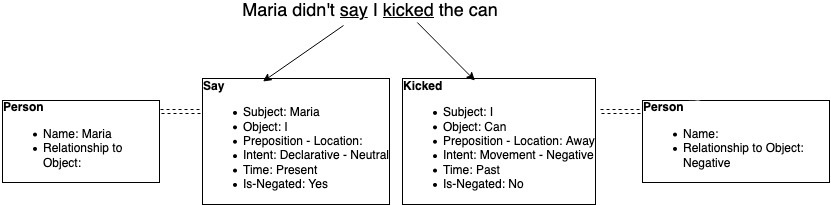
\includegraphics[height=6cm]{Original Maria.jpg}
	\caption{Frame representation of the sentence "Maria didn't say I kicked the can." Frames originally built around verbs.}
	\label{fig:flowchart}
\end{figure}
%First, explain how an AI agent might use the principles of Understanding to make sense of that sentence. As part of this, provide a frame representation of this sentence.
\subsection{Emphasis Changing Frame Representation}
If the sentence had different emphasis placed on it, such as "\textbf{Maria} didn't..." or "...say I \textbf{kicked}...", how could our frames change value? For the first example with the emphasis being on Maria (see Figure 6 below), the primary noun or the noun in the subject case, then the frame will actually remove Maria as the subject for "say" since the word "didn't" negates Maria's place as the primary subject. In this case the frame for say will have an empty Subject, the is-negated slot flips to "No" because someone or something did say that "I kicked the can", and the sub frame of person will change from a filled name slot to an empty slot.
\begin{figure}[h]
	\centering
	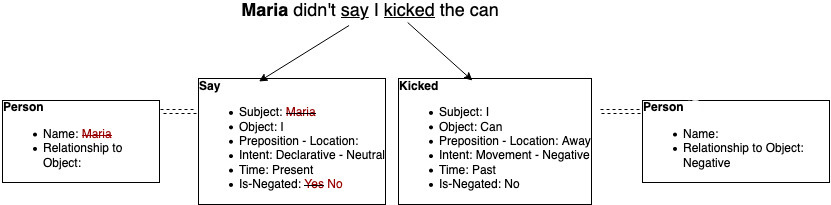
\includegraphics[height=6cm]{Emphasis Maria.jpg}
	\caption{Emphasis on "Maria" places negates Maria being the subject for the Say frame.}
	\label{fig:flowchart}
\end{figure}

\begin{figure}[h]
	\centering
	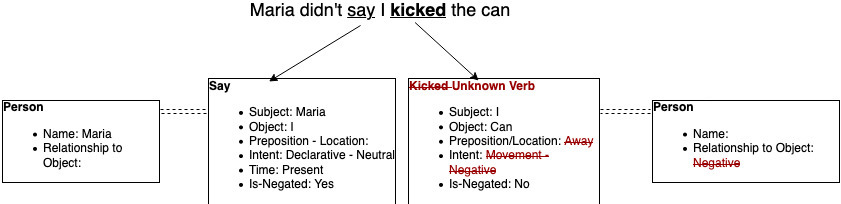
\includegraphics[height=6cm]{Emphasis Kicked.jpg}
	\caption{Emphasis on "kicked" negates the entire "kick" frame into an unknown verb frame.}
	\label{fig:flowchart}
\end{figure}

When the emphasis is instead on "kicked" then there is question for what the verb / action between the direct object (I) and the indirect object (the can) in the sentence. As for how this changes the frame, it negates the Kicked frame entirely into an unknown verb. At that point we can still make assumptions about subject, and object (and therefore the subframes can still hold true for the nouns such as the Person frame in Figure 7 for I). However, an AI agent would then be unable to determined the values for the Preposition/Location slot since those can only be filled in based on default fillers implied by the verb or by direct prepositions in the sentence, as well as the intent slot since that also receives a default-filler based on the action verb used.
%Second, imagine that the sentence had a different emphasis placed on it. “Maria didn’t say I kicked the can”, for example, implies that while someone said I kicked the can, Maria wasn’t the one who said that. “Maria didn’t say I kicked the can” implies while Maria said I did something to the can, she didn’t say I kicked it. Emphasizing any individual word changes the implication of the sentence.

%Explore how the AI agent might be able to understand how different emphases alter the meaning of the sentence. What additional knowledge or abilities would it need to have? As part of this, provide a frame representation that captures these new understandings. You must provide frame representations for at least two different interpretations of the sentence, but you may provide more.
\subsection{Literal or Figurative}
But what of the idiom "kicked the can"? It means to put off work or an action until a later time. How would an AI agent be able to distinguish between the literal and figurative meaning behind the term? An AI agent may use the concepts from "Learning by Recording Cases" where frames for common idioms are included as part of the AI systems working memory. If the frame is "close enough" based on a predetermined threshold (i.e., nearest neighbor but slot differences of 2 slots or less), then the identified frame will inherit the slot values for the "idiom" frame. So in the case for "kicked the can" figuratively the frame should change the Object slot to Time, the Intent to "Declarative - Neutral".
%Finally, discuss how an AI agent might be able to infer whether this sentence is to be taken literally or figuratively. How would an AI agent decide whether the statement describes a literal can or the figurative idea of putting work off for a later date?
\section{Question \#3 - Toronto Declaration}
The Toronto Declaration was established in 2018 as a guiding document for protecting individual rights and preventing discrimination within machine learning and AI systems. The major sections of the document included the Preamble, Using the Framework, Duties of States, Responsibilities of Private Sector Actors, and Right to an Effective Remedy.
\subsection{Summary}
%The Preamble...
The Preamble for the Toronto Declaration lays the groundwork for why a Declaration needs to be established in the first place. Machine Learning systems, without proper forethought, monitoring, and auditing can exacerbate issues of equality and discrimination. These human rights need to have a proper framework for use in machine learning and AI systems as it pertains to all development and uses by the state, and private actors. Additionally there needs to be a system in place to remedy abuses of these human rights within machine learning systems.

%Using the Framework...
The "Using the Framework" section of the Toronto Declaration begins with establishing what the scope for the human right to equality and non-discrimination entails "... such as race, colour, sex, language, religion, political or other opinion, national or social origin, property, birth or other status". It also establishes that there are obligations by both the state and private entities to protect said human rights.

%Duties of States...
The "Duties of States", according to the Declaration, include responsibilities around the state use of machine learning systems that include identifying risks, ensuring transparency and accountability, and enforcing oversight. The state must also promote diversity, and hold private entities accountable.

%Responsibilities of Private Sector Actors...
The "Responsibilities of Private Sector Actors" include the process of exercising the "human rights due diligence" process that includes i) identifying potential discriminatory outcomes, ii) taking action to prevent and mitigate discrimination, and iii) submit high-risk systems for potential equality and discrimination abuses for third-party audits.

%Right to an Effective Remedy...
Finally, the "Right to an Effective Remedy", posits that states and private entities must have a system in place to allow for transparency within machine learning systems as well as methods to hold abuses of the human rights accountable.
% Research the Toronto Declaration. Summarize each of its top-level sections (the Preamble, Using the Framework…, Duties of States, Responsibilities of Private Sector Actors, and Right to an Effective Remedy).
\subsection{Trade-Offs}
Advantages of Toronto Declaration...

Disadvantages of Toronto Declarations...
% Second, analyze the trade-offs inherent to the declaration. In following the declaration, what innovations or opportunities may be lost? If the declaration were discarded, what risks would there be to citizens?
\subsection{Opinion}

% Third, determine your stance on the Toronto Declaration. What do you agree with? What do you disagree with? What would you remove, what would you keep, and what would you add?
\section{Question \#4 - AI and Human Augmentation}
% One role that futurists predict robotics and artificial intelligence will play in the future is human augmentation. Human physical abilities may be augmented with exoskeletons or robotic implements, and human cognitive abilities may be augmented with cybernetic implants. Some futurists suggest that parts of our bodies and brains could be replaced with technological improvements.

% Consider a thought experiment. There are three individuals in the future: Ethan, Sofia, and Akhila.

% Ethan, a mountain climbing enthusiast specializing in conquering the highest peaks in the solar system, decides to wholly embrace the physical augmentations available at the time. First, he opts to have his legs replaced by state-of-the-art robotic legs that never tire and can run several times faster than a typical person. Then, he replaces his arms with the industry standard reconfigurable extremities, which allow him to replace his hands with other tools at will. He then is a subject in a late-stage device development for a system that replaces his digestive and respiratory systems with technological alternatives for more convenient energy storage and distribution. Finally, after an accident that irreparably damages the bones in his jaw, he replaces his own face and head with a robotic container. In the end, the only organic part of Ethan remaining is his brain, housed in an otherwise robotic body.

% Sofia, on the other hand, does not opt for any bodily reconfiguration. However, as pilot of commuter starships, the demands on her attention span and working memory are extremely high. She thus undergoes a procedure that augments her frontal lobe. Several years later, new research reveals that the augmentation results in the brain increasingly relying on the implant, and thus ultimately she must have her frontal lobe and temporal lobe replaced by equivalent technological analogues. Later, to allow her to use a new generation of cybernetically-connected ship controls, she has her parietal and occipital lobes replaced; her original lobes are scanned to ensure its content is preserved in their new replacements, which also allow for direct API connections. In the end, Sofia’s entire brain has been replaced, though the content of her original brain was scanned and included in each replacement. Ethan and Sofia are opposites of one another; anything that Ethan had replaced, Sofia retained, and vice versa.

% Finally, Akhila, Ethan’s mountain climbing partner as well as Sofia’s regular copilot, ultimately undergoes all the same procedures as both of her friends, in roughly the same sequence. In the end, nothing organic is left from Akhila’s original body and brain.
\subsection{Identity Definition}
\subsection{Threshold for Identity}
\subsection{Identity for Ethan, Sofia, Akhila Thought Experiment}
% After all the procedures have been completed, who is still the same person they were originally? Is Ethan still Ethan? Is Sofia still Sofia? Is Akhila still Akhila? If any are not still the person they began as, at what point did they cease to be that person? Why?

% Provide your answers to the above questions, and argue for your perspective. In your argument, consider the significance of the narrative: would it be different if Ethan had his entire body replaced at once, or if an entire copy of Akhila was built from a backup after a tragic accident? Your argument should not be purely opinion-based; you should provide definitions for relevant concepts regarding personhood and identity, and construct your argument from those definitions.

\section{Typography}
All text in JDF should be set in the Palatino typeface. It is available practically everywhere as a system font: Microsoft ships a version called \emph{Palatino Linotype}, and Apple uses a version simply called \emph{Palatino}. Those without either can look for \emph{Book Antiqua} in their fonts list or download \href{https://www.ctan.org/tex-archive/fonts/tex-gyre/opentype}{\TeX\ Gyre Pagella} from CTAN. They all come in regular and bold weights with matching italics.

\subsection{Body text}
Body text is set in the regular weight at 11 points with 17 points of line spacing, and 8.5 points of spacing added after each paragraph. It should be justified with hyphenation enabled where available. Paragraphs should not be indented. These styles can be automatically applied using the \emph{Normal} paragraph style.

\textbf{Bold} and \textit{italics} should be used for emphasis. Hyperlinks may be inserted in the text, as well as {\tt in-line code}, superscripts\textsuperscript{ like this}, and subscripts\textsubscript{ like this}.

\subsection{Title \& subtitle}
The paper title should be set in the regular weight at 17 points with 22 points of line spacing, centered at the top of the first page. The title may span up to three lines. For typical assignments, the document title may be as simple as “Assignment 1” More specialized assignments may warrant more unique paper names, like “A Proposal to Create a New Document Format.”

The author’s name and email should come next unless you want to or were asked to submit anonymously, in which case this can be omitted. They should be set in the same size and weight as body text, centered. These styles can be applied using the \emph{Title} and \emph{Subtitle} paragraph styles.

\subsection{Abstract}
If your paper requires an abstract, it should be placed at the top of the first page underneath the title block, preceded by the word \emph{Abstract} in bold italic. An extra 0.5" should be added to both sides. Not all papers require abstracts; only those that would benefit from a high-level summary of the project or its background.

\subsection{Headings}
Headings should all be set in the same size as body text (11 pt) in bold. With the exception of \emph{Heading 1}, they should all have 8.5 pt of space before and after. They should be hierarchically numbered: Word, Pages, and \LaTeX\ will do this automatically when you use the appropriate paragraph styles, but Google Docs users will need to number their headings manually. Headings should not span more than one line.

\subsubsection{Heading 1}
Heading 1 should be set in all caps, with letterspacing expanded by 0.66 points (6\%). It should have 11 points of space added before and 8.5 points of space added after.

\subsubsection{Headings 2\,–\,4}
Besides \emph{Heading 1}, which is set in caps, headings should always use sentence case (i.e., first word capitalized) rather than title case; after all, they are not titles. \emph{Heading 2} should be set in bold roman (upright), and \emph{Heading 3} should be set in bold italics. The use of headings beyond \emph{Heading 3} is discouraged.

\subsubsubsection{Heading 4}\emph{Heading 4} is provided as a run-in sidehead. Like \emph{Heading 3}, it is set in bold italics, but it should be followed by an em dash and flow right into the text, as seen at the beginning of the current paragraph. It should be used more as a list style than a heading style, e.g. to set off a list of principles in a heuristic evaluation.

\subsection{Page layout}
JDF uses the US Letter paper size (8.5" x 11"). It has a top margin of 1", and bottom and side margins of 1.5". This yields a text block of 5.5" x 8.5", which is exactly \(\frac{1}{2}\) the size of the page, divided lengthwise.

The page number should be included in the bottom margin, 1" from the bottom of the page – this creates symmetry with the top margin. No other elements should be placed in the margins.

\section{Presentational elements}
You are encouraged to use presentational elements liberally, as long as they add to the clarity of your submissions. They often require less space and fewer accompanying words to explain a given concept, and do a far better job of it.

\subsection{Figures}
Figures should always be centered on the page, although they may also take up the entire width and height of the text block. Figures should always be referenced in the text, and they should include a descriptive caption. Figures may also be equations, diagrams, or other kinds of content.

If your figure includes a white background (e.g. an interface design or graph), it may aid legibility to add a \(\frac{1}{4}\)-point black border.

\begin{figure}[h]
	\centering
	\includegraphics[height=6cm]{Figures/flowchart.png}
	\caption{Make sure your flowcharts are more useful than this one. Source: \href{https://xkcd.com/1195/}{XKCD}.}
	\label{fig:flowchart}
\end{figure}

Figure captions should be centered beneath the corresponding figure. The label (e.g. “Figure 1”) should be set in bold italics followed by an em dash, and the entire caption should be 8.5 pt with 14 pt of line spacing. The \emph{Figure Caption} style in Word will number your figures automatically. If need be, you may have one figure caption corresponding to consecutive figures and use either locational descriptors (e.g. “top left,” “middle”) or labels (e.g. “A”, “B”) to map parts of the caption to parts of the figure. Make sure captions fall on the same page as the corresponding figure or table; you may rearrange text to make this work.

In Word, you may need to either change the image’s text wrap settings to “Top and Bottom” or change the line spacing of the image to 1.0.

\subsection{Tables}
You have freedom to format tables in the way that works best for your data. Generally, text should be left-aligned and numbers should be right-aligned or aligned at the decimal – you can do this using a custom tab stop. The default table style (shown below) reduces the text size to be equal to the caption text.

Table captions should be formatted the same way as figure captions, but they should be placed above the table. The popular mnemonic for this is: figures at the foot, tables at the top. Like figures, tables should not exceed the margins and should be centered on the page.

\begin{table}[h] % [h] forces the table to be output where it is defined in the code (it suppresses floating)
	\caption{Mathematical constants. Notice how the approximations align at the decimal.}
	\small % Reduce font size
	\centering % Centre the table
	\begin{tabular}{L{0.17\linewidth} C{0.12\linewidth} L{0.17\linewidth} L{0.4\linewidth}}
		\textbf{Name} & \textbf{Symbol} & \textbf{Approximation} & \textbf{Description} \\
		\toprule[0.5pt]
		Golden ratio & $\phi$ & 1.618 & Number such that the ratio of " to the number is equal to the ratio of its reciprocal to 1\\
		\midrule
		Euler's number & $e$ & 2.71828 & Exponential growth constant\\
		\midrule
		Archimedes' constant & $\pi$ & 3.14 & The ratio between circumference and diameter of a circle\\
		\midrule
		One hundred & A+ & 100.00 & The grade we hope you’ll all earn in this class\\
	\end{tabular}
\end{table}

\subsection{Additional elements}
There are additional elements you may want to include in your paper, such as in-line or block quotes, lists, and more. For other content types not covered here, you have flexibility in determining how it should be used in this format.

\subsubsection{Quotes}
If you would like to quote an outside source, you may do so with quotation marks followed by a citation. If a quote is fewer than three lines, you may write it in-line. It is acceptable to replace pronouns with their target in brackets for clarity. For example, “Heavy use of peer grading would compromise [the school’s] reputation” (Joyner, 2016). If a quote exceeds three lines, you should set it as its own paragraph with 0.5” side margins, using the Blockquote style.

\begin{quotation}
	\noindent “Whether or not the grades generated by peers are reliably similar to grades generated by experts is only one factor worth considering, however. Student perception is also an important factor. A recent study indicated that reliance on peer grading is one of the top drivers of high MOOC dropout rates. This problem may be addressed by reintroducing some expert grading where possible.” %\citep{joyner2016}
\end{quotation}

\subsubsection{Lists}
Bulleted and numbered lists are indented 0.5" from the left margin, with the bullet or number hanging in the margin by 0.25" (the default format).

Bullet points:

\begin{itemize}
	\item First bullet point item
	\item Second bullet point item
\end{itemize}

Numbered list:

\begin{enumerate}
	\item First numbered item
	\item Second numbered item
\end{enumerate}

\section{Procedural elements}
\subsection{In-line citations}
Articles or sources to which you refer should be cited in-line with the authors’ names and the year of publication.\footnote{In-line citations are preferred over footnotes, and we favor APA citation format for both in-line citations and reference lists. Refer to the Purdue Online Writing Lab, or follow the above examples. Footnotes should use 8.5 point text with 14 point line spacing.} The citation should be placed close in the text to the actual claim, not merely at the end of the paragraph. For example: students in the OMSCS program are older and more likely to be employed than students in the on-campus program \citep{joyner2017}. In the event of multiple authors, list them. For example: research finds sentiment analysis of the text of OMSCS reviews corresponds to student-assigned ratings of the course \citep{newman2018}. You may also cite multiple studies together. For example: several studies have found students in the online version of an undergraduate CS1 class performed equally with students in a traditional version (\cite{joyner2018a}; \cite{joyner2018b}). If you would like to refer to an author in text, you may also do so by including the year (in parentheses) after the author’s name in the text. If a publication has more than 4 authors, you may list the first author followed by ‘et al.’ For example: \citeauthor{joyner2016} (\citeyear{joyner2016}) claim that a round of peer review prior to grading may improve graders’ efficiency and the quality of feedback given. This applies to parenthetical citations as well, e.g. \citep{joyner2016}.

\subsection{Reference lists}
References should be placed at the end of the paper in a dedicated section. Reference lists should be numbered and organized alphabetically by first author’s last name. If multiple papers have the same author(s) and year, you may append a letter to the end of the year to allow differentiated in-line text (e.g. Joyner, 2018a and Joyner, 2018b in the section above). If multiple papers have the same author(s), list them in chronological order starting with the older paper. Only works that are cited in-line should be included in the reference list. The reference list does not count against the length requirements.

\section{References}
\printbibliography[heading=none]

\section{Appendices}
You may optionally move certain information to appendices at the end of your paper, after the reference list. If you have multiple appendices, you should create a section with a \emph{Heading 1} of “Appendices.” Each appendix should begin with a descriptive \emph{Heading 2}; appendices can thus be referenced in the body text using their heading number and description, e.g. “Appendix 5.1: Survey responses.” If you have only one appendix, you can label it with the word “Appendix” followed by a descriptive title, e.g., “Appendix: Survey responses.”

These appendices do not count against the page limit, but they should not contain any information required to answer the question in full. The body text should be sufficient to answer the question, and the appendices should be included only for you to reference or to give additional context. If you decide to move content to an appendix, be sure to summarize the content and note it in relevant place in the body text, e.g., “The raw data can be viewed in \emph{Appendix 5.1: Survey responses}.”

\end{document}